\chapter{Executive Summary}
\label{ch:fdsp-execsum}

\section{Introduction}
\label{sec:fdsp-exec-introduction}
%Broad physics motivation for the detector.


The overriding physics goals of the \dword{dune} are the search for leptonic \dword{cp} violation, the search for nucleon decay as a signature of a Grand Unified Theory underlying the Standard Model, and the observation of neutrino bursts from supernovae. Central to achieving this physics program is the construction of a detector that combines the many-kiloton fiducial mass necessary for rare event searches with sub-centimeter spatial resolution in its ability to image those events, allowing us to identify the signatures of the physics processes we seek among the numerous backgrounds. The \dword{sp} \dword{lartpc}~\cite{Rubbia:1977zz} allows us to achieve these dual goals, providing a way to read out with sub-centimeter granularity the patterns of ionization in $\SI{10}{kt}$ volumes of \dword{lar} resulting from the $O(\SI{1}{MeV})$ interactions of solar and supernova neutrinos up to the $O(\SI{1}{GeV})$ interactions of neutrinos from the \dword{lbnf} beam.

To search for leptonic \dword{cp} violation, we must study \nue appearance in the \dword{lbnf} \numu beam. This requires the ability to separate electromagnetic activity induced by \dword{cc} \nue interactions from similar activity arising from photons, such as photons from $\pi^{0}$ decay. Two signatures allow this: photon showers are typically preceded by a gap prior to conversion, characterized by the \SI{18}{cm} conversion length in \dword{lar}; and the initial part of a photon shower, where an electron-positron pair is produced, has twice the $\mathrm{d}E/\mathrm{d}x$ of the initial part of an electron-induced shower. To search for nucleon decay, where the primary channel of interest is $p\rightarrow K^{+}\overline{\nu}$, we must identify kaon tracks as short as a few centimeters. It is also vital to accurately fiducialize these nucleon-decay events to suppress cosmic-muon-induced backgrounds, and here the detection of argon-scintillation photons is important for determining the time of the event. Detecting a \dword{snb} poses different challenges: those of dealing with a high data-rate and maintaining the high detector up-time required to ensure we do not miss one of these rare events. The signature of a \dword{snb} is a collection of MeV-energy electron tracks a few centimeters in length from \dword{cc} $\nu_{e}$ interactions, spread over the entire detector volume. To fully reconstruct a \dword{snb}, the entire detector must be read out, a data-rate of up to $\SI{2}{\tera\byte/\second}$, for \SIrange{30}{100}{s}, including a $\sim\!\SI{4}{s}$ pre-trigger window.

In this Executive Summary, we give an overview of the basic operating principles of a \dword{sp} \dword{lartpc}, followed by a description of the \dword{dune} implementation. We then discuss each of the sub-systems separately, connecting the high-level design requirements and decisions to the overriding physics goals of \dword{dune}.

\section{The Single-Phase Liquid Argon Time-Projection Chamber}
\label{sec:fdsp-exec-splar}
%General operating principle

\begin{dunefigure}[The single-phase liquid argon time-projection chamber]{fig:LArTPC}
{The general operating principle of the single-phase liquid argon time-projection chamber.}
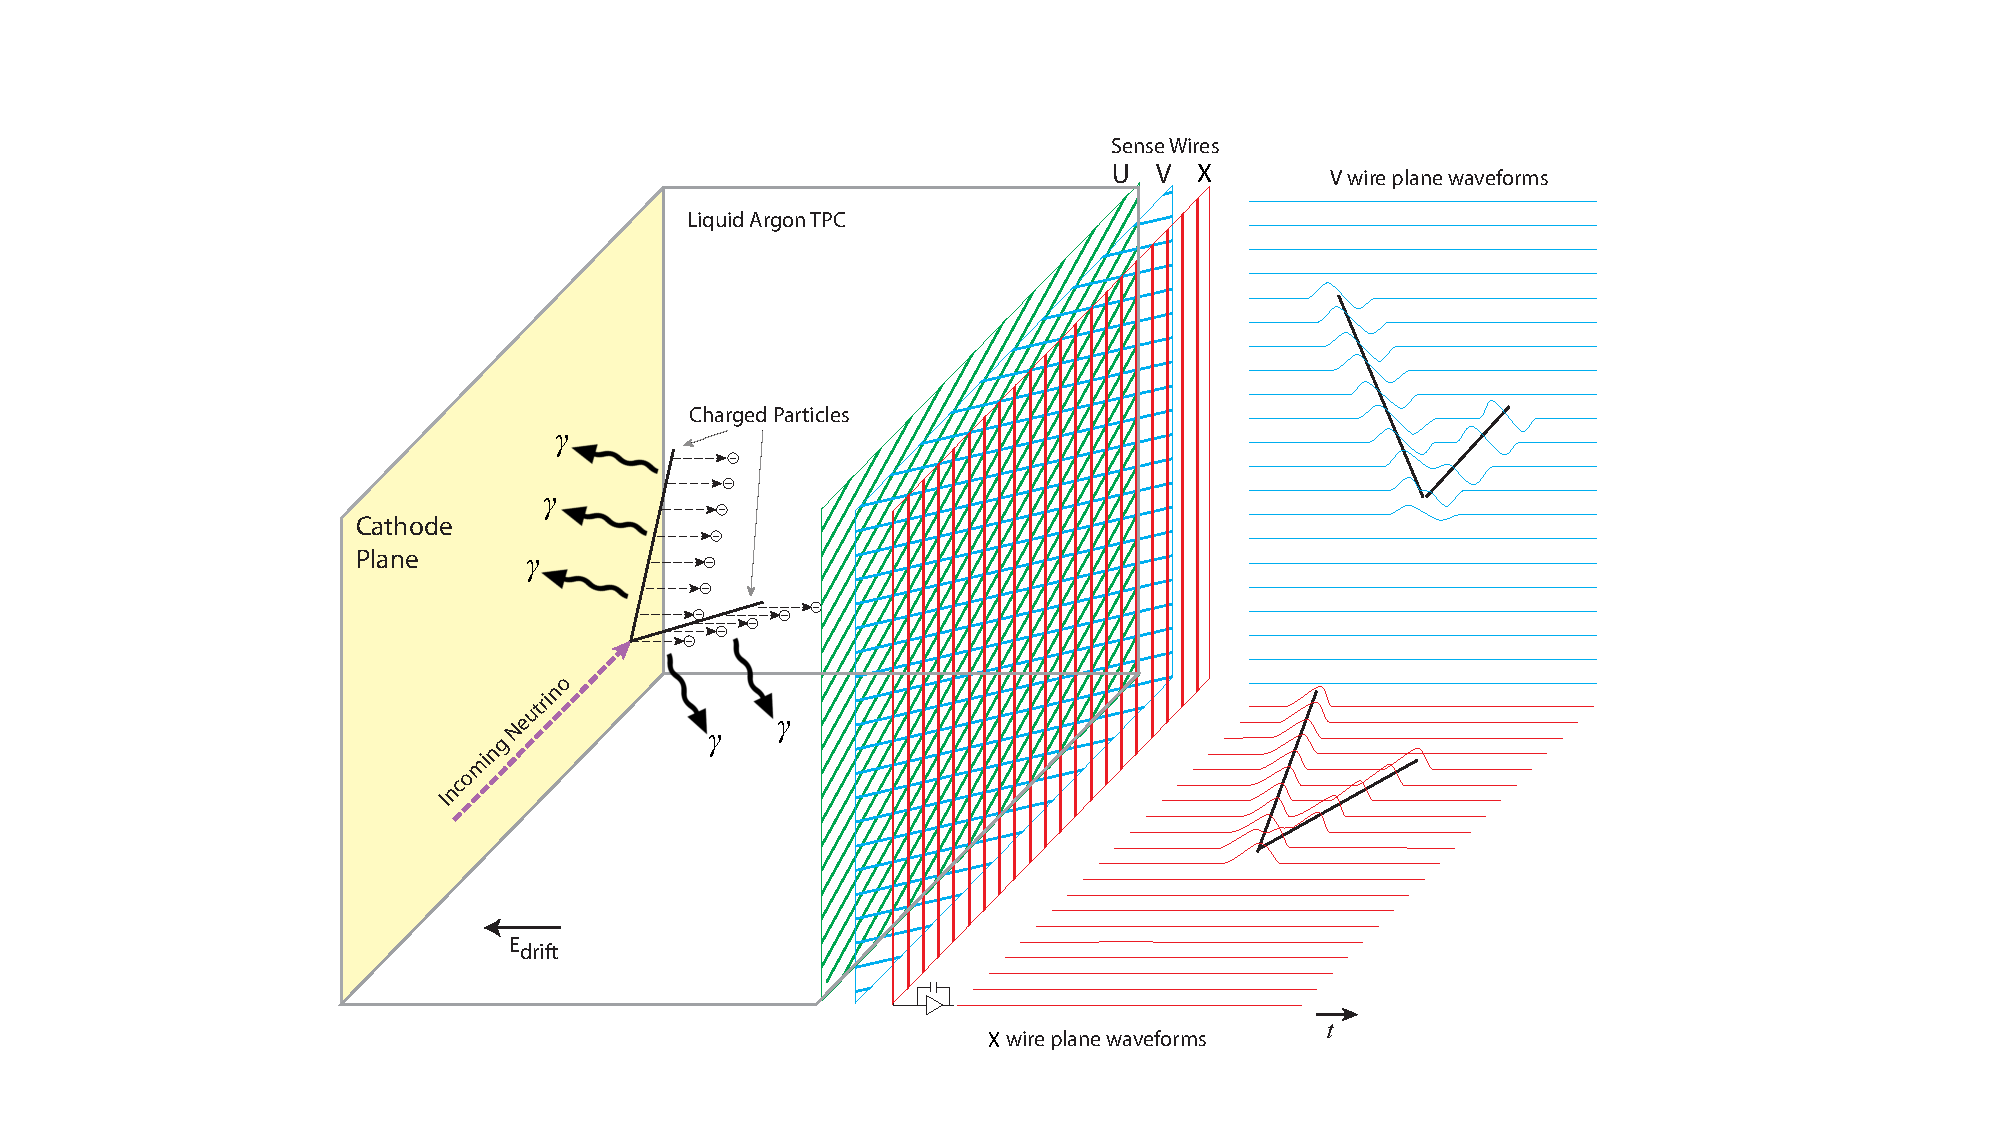
\includegraphics[trim={5cm 0 5cm 0},clip,width=0.8\textwidth]{graphics/TheBoPicture.pdf}
\end{dunefigure}

Figure~\ref{fig:LArTPC} shows the general operating principle of a \dword{sp} \dword{lartpc}, as has been previously demonstrated by
%\fixme{I don't have a dword for ICARUS. All the others are in the common glossary.} 
ICARUS~\cite{Icarus-T600},
\dword{argoneut}~\cite{Anderson:2012vc}, \dword{microboone}~\cite{microboone}, \dword{lariat}~\cite{Cavanna:2014iqa}, and \dword{protodune}~\cite{Abi:2017aow}. A large volume of \dword{lar} is subjected to a strong electric field of a few hundred volts per centimeter. Charged particles passing through the detector ionize the argon atoms, and the ionization electrons drift in the electric field to the anode wall on a timescale of milliseconds. This anode consists of layers of active wires forming a grid. The relative voltage between the layers is chosen to ensure all but the final layer are transparent to the drifting electrons, and these first layers produce bipolar induction signals as the electrons pass through them. The final layer collects the drifting electrons, resulting in a monopolar signal.

\dword{lar} is also an excellent scintillator, emitting \dword{vuv} light at a wavelength of \SI{126.8}{\nano\meter}. This fast scintillation light, which crosses the detector on a timescale of nanoseconds, is shifted into the visible and collected by \dword{pd} devices. The \dword{pd}s can provide a $t_{0}$ determination for events, telling us when the ionization electrons begin to drift. Relative to this $t_{0}$, the time at which the ionization electrons reach the anode allows reconstruction of the event topology along the drift direction, which is crucial to fiducialize nucleon-decay events and to apply drift corrections to the ionization charge.

The pattern of current observed on the grid of anode wires provides the information for reconstruction in the two coordinates perpendicular to the drift direction. A closer spacing of the wires, therefore, results in better spatial resolution, but, in addition to increasing the cost of the readout electronics due to the additional wire channels, a closer spacing worsens the signal-to-noise of the ionization measurement because the same amount of ionization charge is now divided over more channels. Signal-to-noise is an important consideration because the measurement of the ionization collected is a direct measurement of the $\mathrm{d}E/\mathrm{d}x$ of the charged particles, which is what allows us to perform both calorimetry and particle identification.

\section{The \dshort{dune} Single-Phase Far Detector Module}
\label{sec:fdsp-exec-dunefd}
%Explain 10 kt modules, and then explain the overall setup.
%As part of this, explain the main design parameters and how they relate to the physics drivers.

\begin{dunefigure}[A $\SI{10}{\kilo\tonne}$ DUNE Far Detector single-phase module.]{fig:DUNESchematic}{A 10 kt DUNE Far Detector single-phase module, showing alternating anode (A) and cathode (C) planes, as well as the field cage that surrounds the drift regions between the anodes and cathodes.}
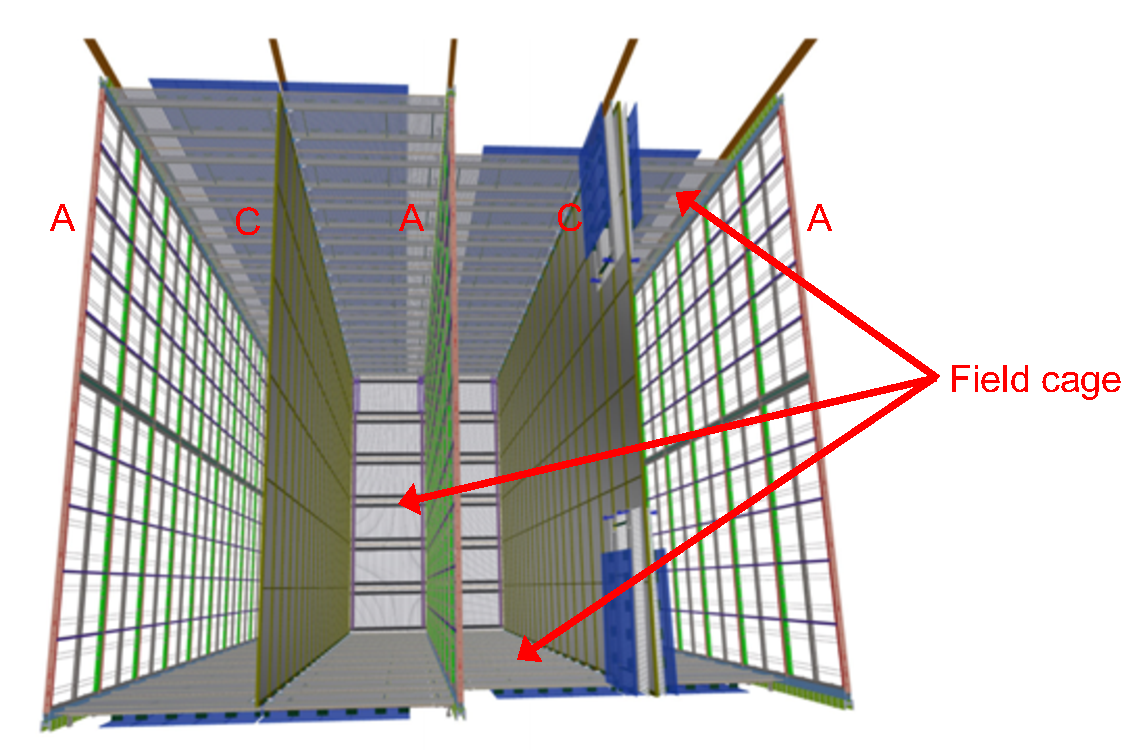
\includegraphics[width=0.8\textwidth]{DUNESchematic.pdf}
\end{dunefigure}

The DUNE \dword{sp} \dword{lartpc} consists of \SI{10}{\kilo\tonne} modules, contributing to the full \SI{40}{\kilo\tonne} \dword{fd} mass. Figure~\ref{fig:DUNESchematic} shows a \SI{10}{\kilo\tonne} module. Inside a cryostat of outer dimensions $\SI{62}{\meter}\times \SI{19}{\meter}\times \SI{18}{\meter}$ (shown in Fig.~\ref{fig:Cryostat}), four $\SI{3.5}{\meter}$ drift volumes are created between five alternating anode and cathode walls, each wall having dimensions of $\SI{58}{\meter}\times \SI{12}{\meter}$.

\begin{dunefigure}[A DUNE cryostat.]{fig:Cryostat}{A $\SI{62}{\meter}\times \SI{19}{\meter}\times \SI{18}{\meter}$ outer-dimension cryostat that houses a DUNE \SI{10}{\kilo\tonne} module.}
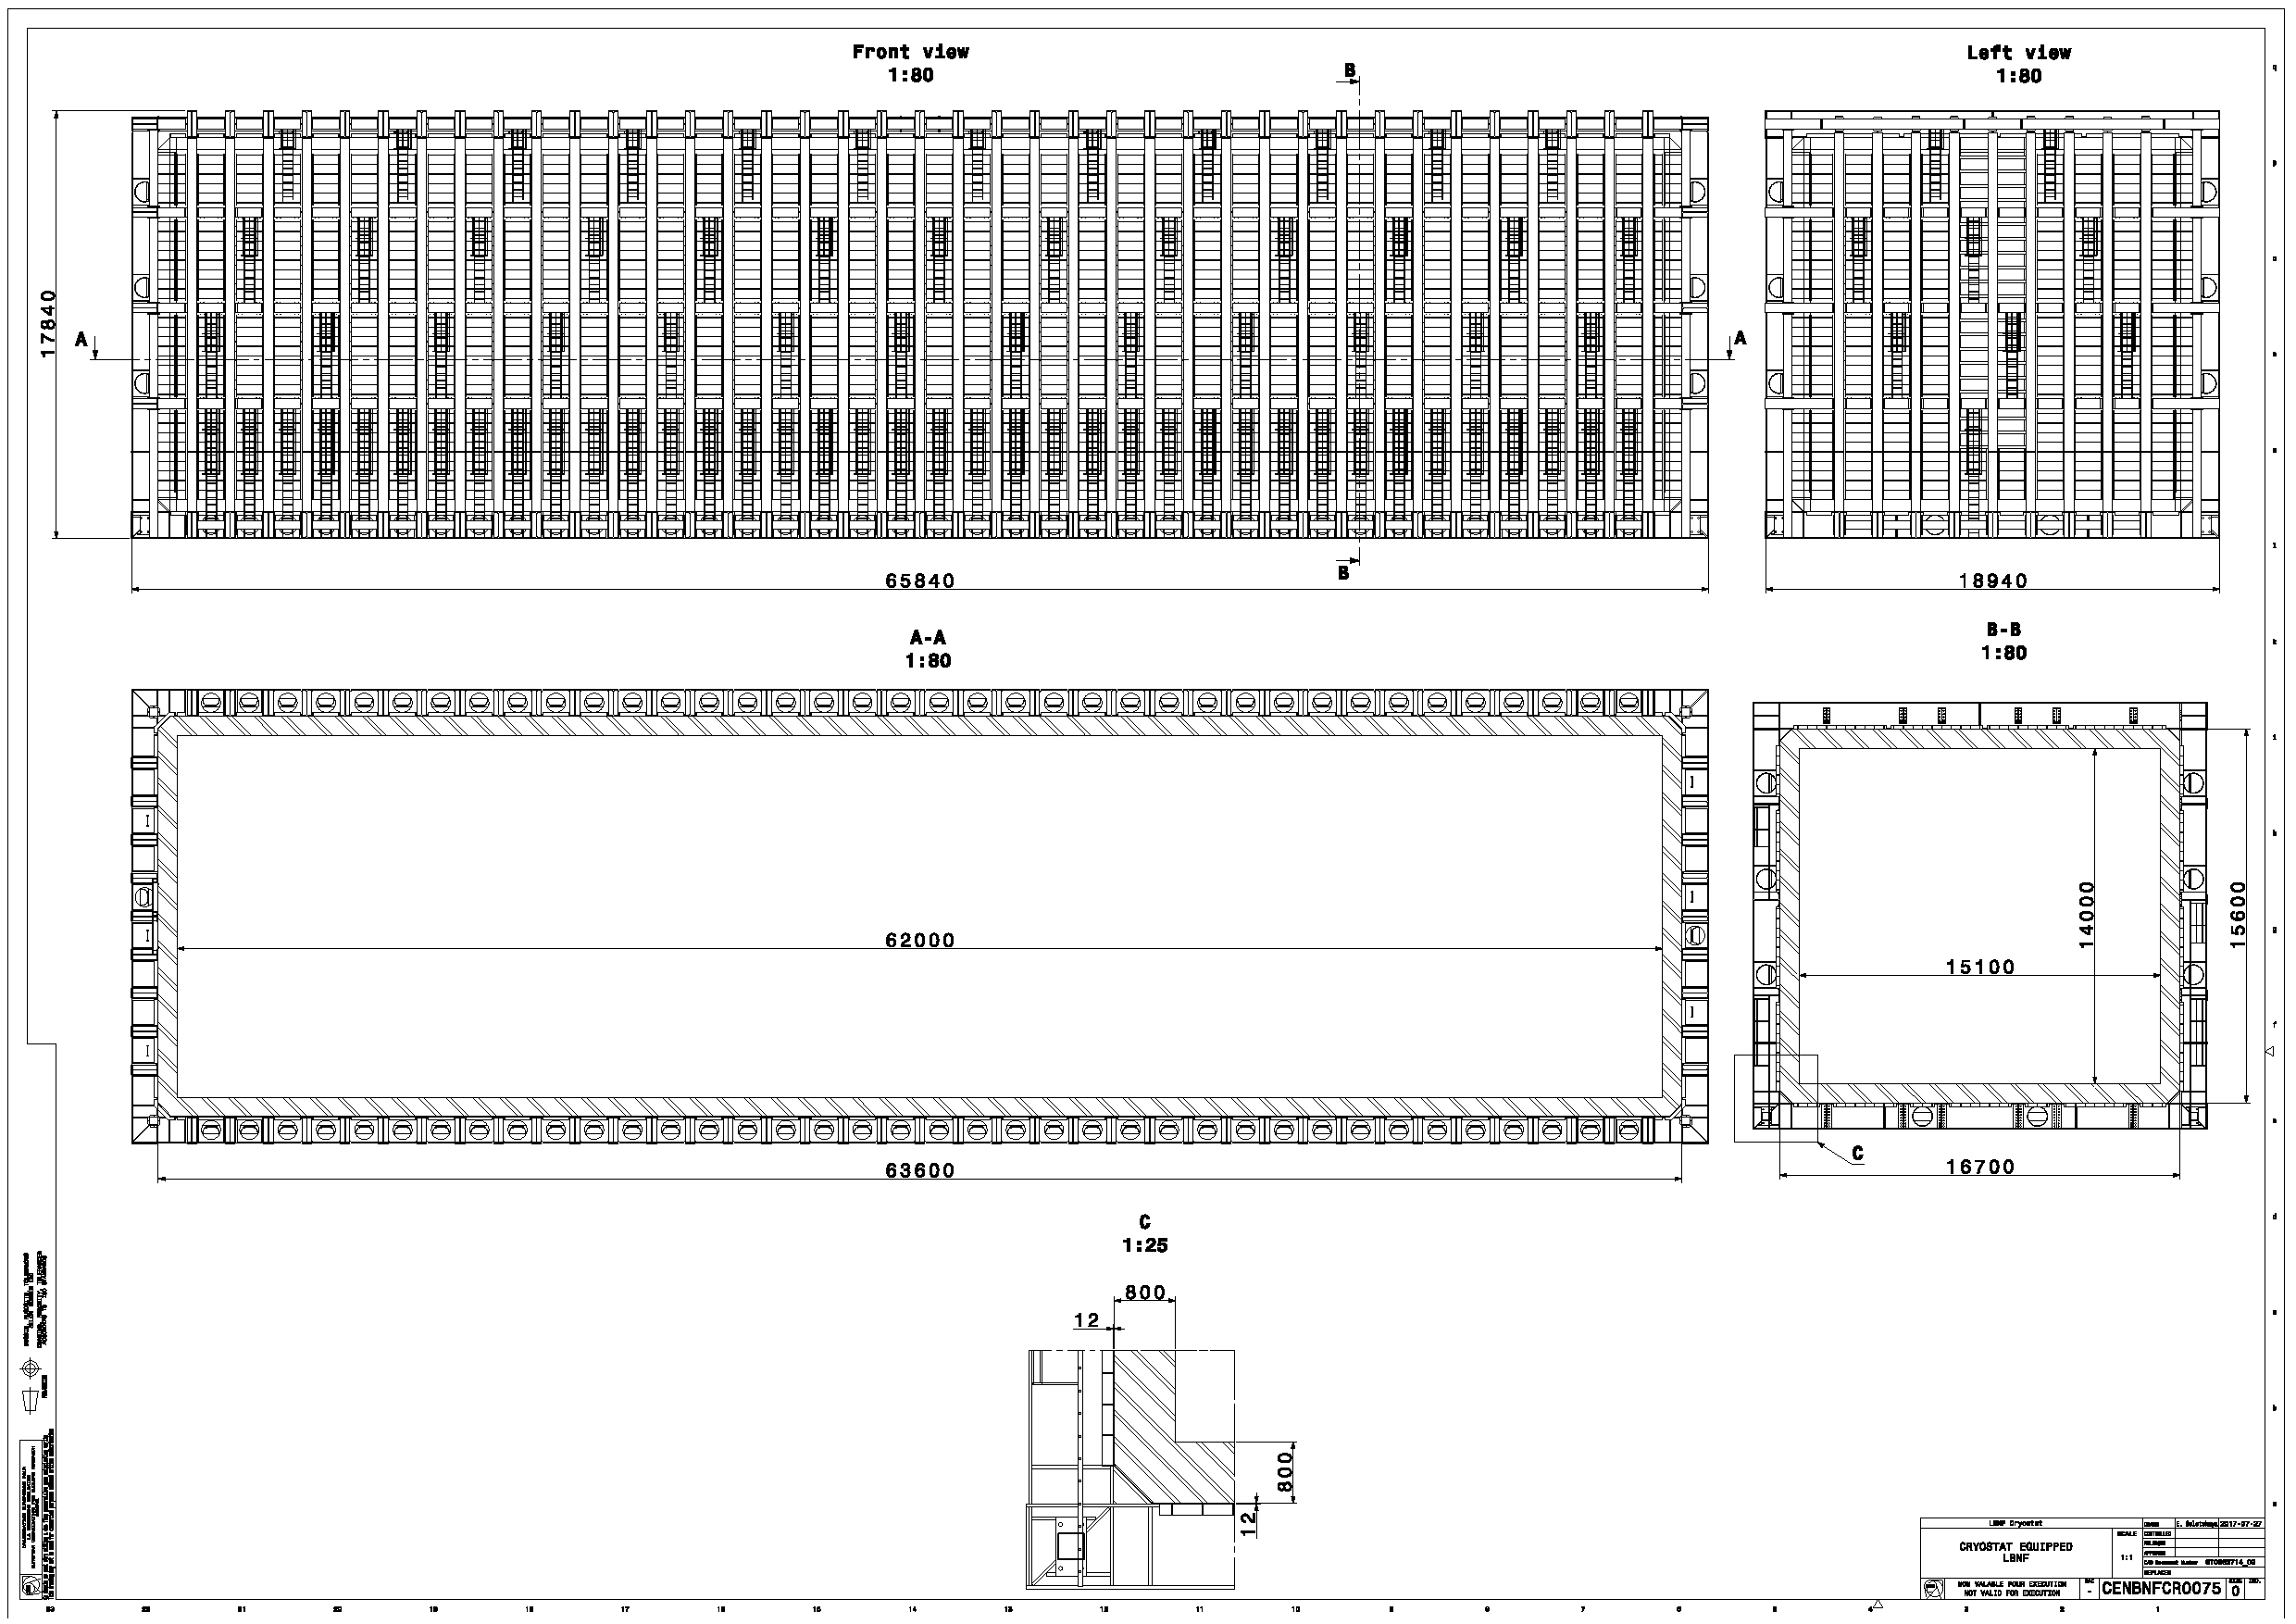
\includegraphics[width=0.8\textwidth]{cryostat.pdf}
\end{dunefigure}

The \dword{fd} is located underground, at the \SI{4850}{\foot} level of the \dword{surf} in South Dakota. The detector is \SI{1300}{\km} from the source of the \dword{lbnf} neutrino beam at \dword{fermilab}; this baseline provides the matter effects necessary for \dword{dune} to determine the neutrino mass hierarchy. The \dword{surf} underground campus is shown in Fig.~\ref{fig:SURFCaverns}. The four \SI{10}{\kilo\tonne} \dword{fd} modules will be located in the two main caverns, which are each \SI{144.5}{\meter} long, \SI{19.8}{\meter} wide and \SI{27.95}{\meter} high. Each cavern houses two \SI{10}{\kilo\tonne} modules, one either side of the central access drift. Between the two caverns is the \dword{cuc}, a \SI{190}{\meter} long, \SI{19.3}{\meter} wide, \SI{10.95}{\meter} high cavern in which many of the utilities and the upstream \dword{daq} reside.

\begin{dunefigure}[A $\SI{10}{\kilo\tonne}$ DUNE Far Detector single-phase module.]{fig:SURFCaverns}{The underground layout of the \dword{surf} laboratory. The two main caverns each hold two \SI{10}{\kt} \dword{fd} modules, one either side of the central access drift. The \dword{cuc} houses utilities and the upstream \dword{daq}.}
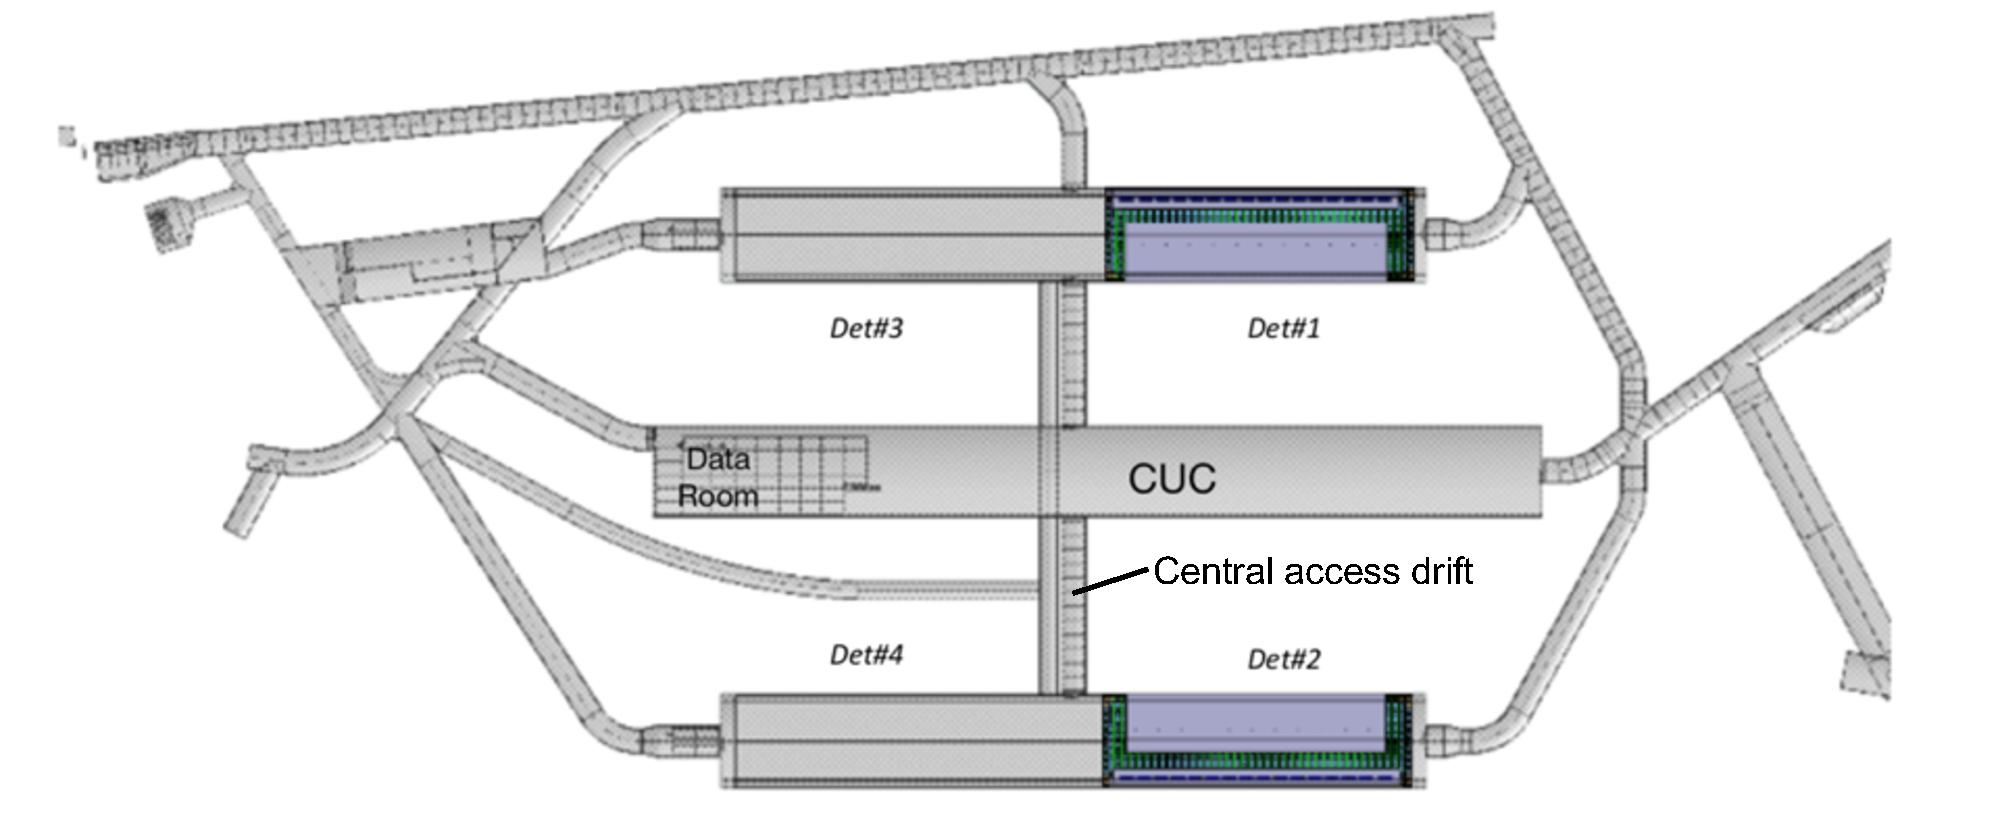
\includegraphics[width=\textwidth]{UndergroundLayout2.pdf}
\end{dunefigure}

Each cathode wall in a module is called a \dword{cpa} array. The \dword{cpa} is the $\SI{1.2}{\meter}\times\SI{4}{\meter}$ panel from which the \dword{cpa} arrays are formed; each \dword{cpa} array contains $150$ \dword{cpa}s. The \dword{cpa} arrays are held at $-\SI{180}{\kilo\volt}$. With the anode walls held close to ground, this results in a uniform \SI{500}{\volt/\centi\meter} electric field across the drift volume. A \dword{fc} surrounds the remaining open sides of the \dword{tpc}, ensuring the field is uniform to better than 1\% throughout the active volume. A typical minimum ionizing particle passing through the argon produces around $60k$ ionization electrons per centimeter, which drift towards the anodes at around $\SI{1.6}{\mm/\micro\second}$; the time taken to drift the full distance from cathode to anode would therefore be around $\SI{2.4}{\milli\second}$.

The anode walls are each made up of 50 \dword{apa} units that are $\SI{6}{\meter}\times\SI{2.3}{\meter}$ in dimension. As shown in Figure~\ref{fig:APAStack}, the \dword{apa}s hang vertically; each anode wall is two \dword{apa}s high and 25 \dword{apa}s wide. The \dword{apa}s are two-sided, with three active wire layers and an additional shielding layer, also called a grid layer, wrapped around them. The wire spacing on the layers is $\sim\!\SI{5}{\mm}$. The collection layer is called the $X$-layer; the induction layer immediately next to that is called the $V$-layer; the next induction layer is the $U$-layer; and the shielding layer is the $G$-layer. $X$-layer and $G$-layer wires are vertical; the $U$- and $V$-layer wires are at $\pm\SI{35.7}{\degree}$ to the vertical.

\begin{dunefigure}[A stack of two anode plane assemblies.]{fig:APAStack}
{Left: two \dword{apa}s linked together to form one unit of an \dword{apa} wall. \dword{pd} bars can be seen installed across the width of the \dword{apa}s. Right: a zoom into the top and bottom ends of the \dword{apa} stack showing the readout electronics, and the centre of the stack where the \dword{apa}s are connected together.}
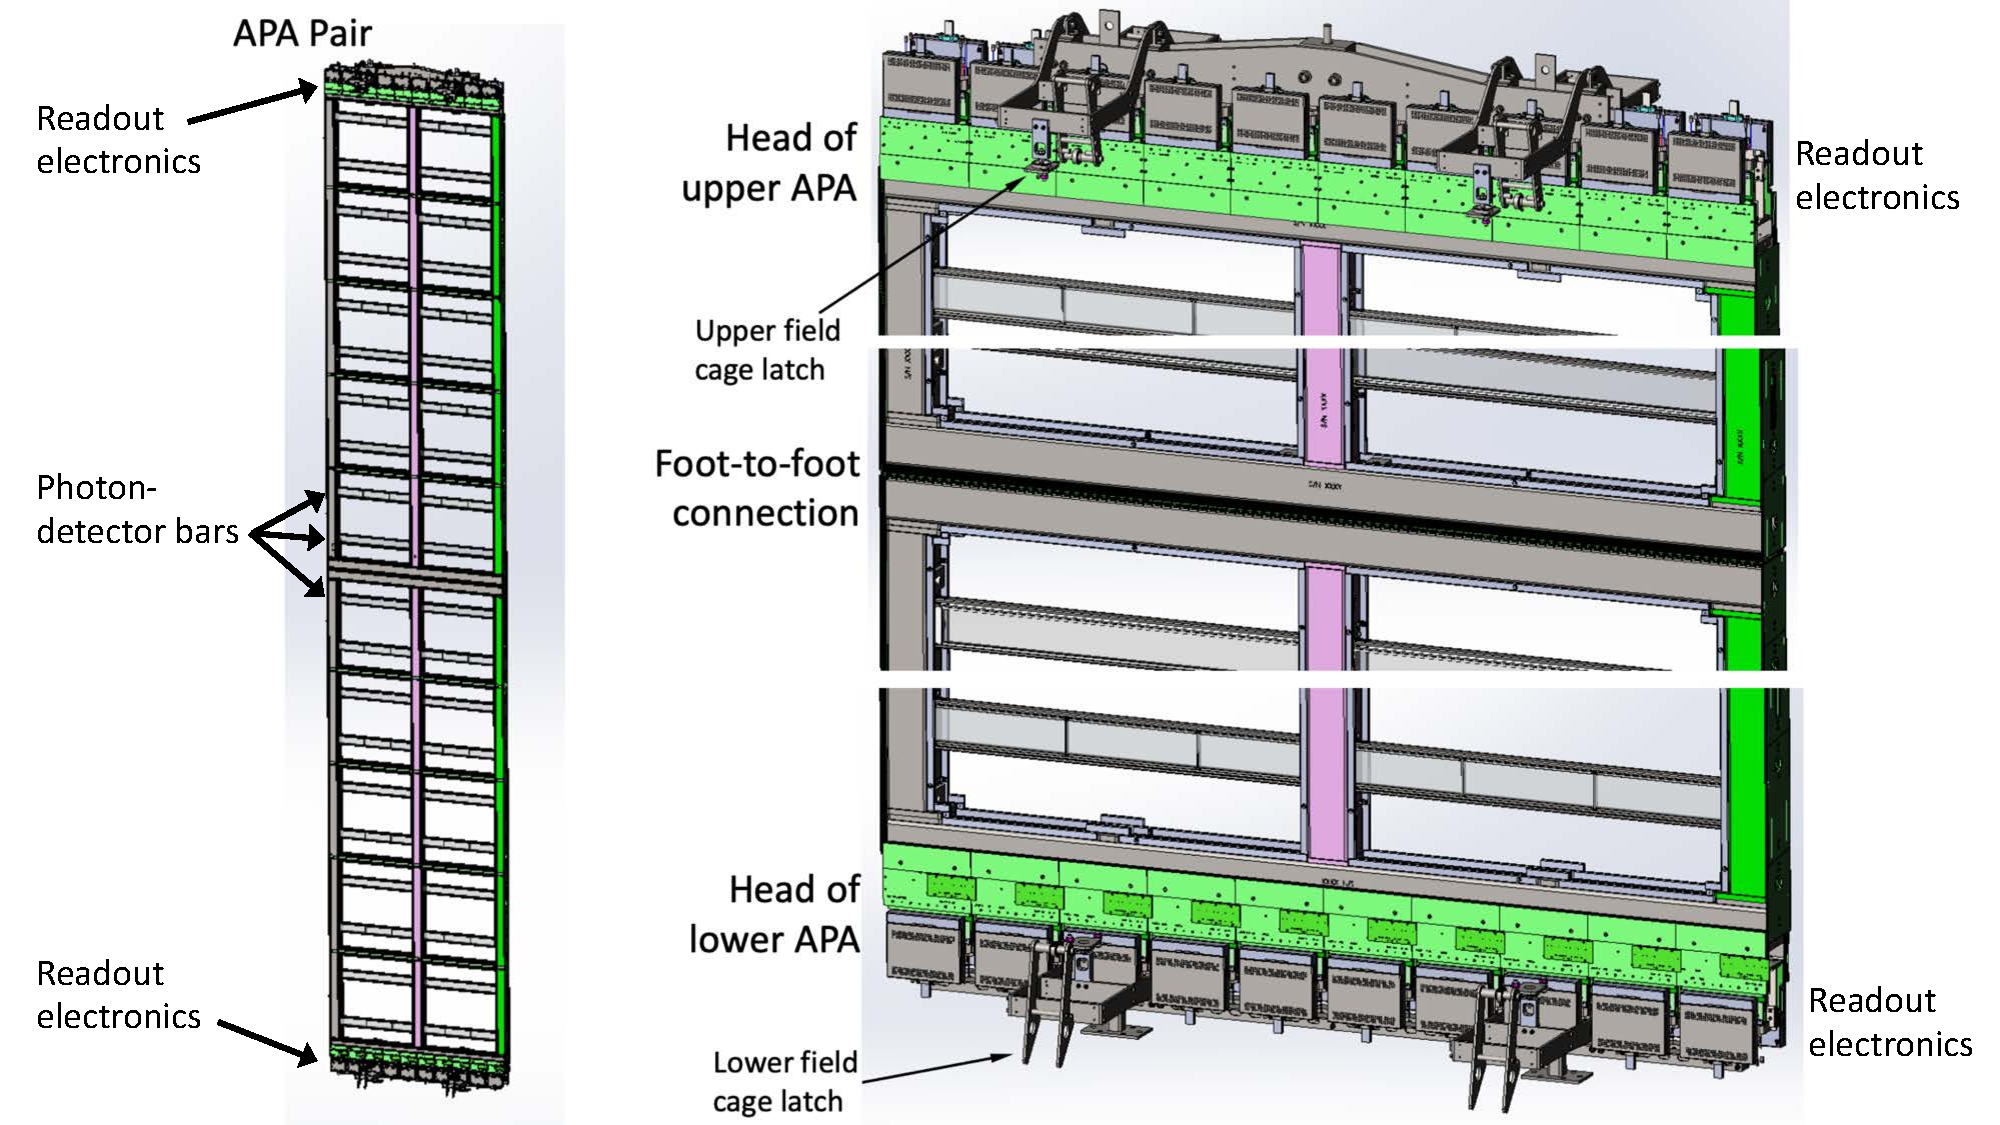
\includegraphics[width=\textwidth]{graphics/APAStack.pdf}
\end{dunefigure}

Readout electronics, called \dword{ce}, are attached to the top end of the top \dword{apa} and the bottom end of the bottom \dword{apa}. These front-end electronics benefit from the low \dword{lar} temperature through the reduction of thermal noise. The front-end electronics shape, amplify, and digitize the signals from the induction and collection wires thanks to a series of three different types of \dword{asic} through which all signals pass.
%On each \dword{apa} are 20 front-end motherboards, on which the \dword{asic}s are mounted, and each motherboard processes the signals from 40 $U$, 40 $V$, and 48 $X$-layer wires.
Cables from the \dword{ce} pass through feedthroughs on the roof of the cryostat; cables from the motherboards on the bottom \dword{apa} pass through the inside of the hollow \dword{apa} frames up to the top.

Once signals from \dword{apa}s leave the cryostat through feedthroughs, they are passed to warm interface boards that put the signals onto \SI{10}{\giga\byte} optical fibers, ten fibres per \dword{apa}, which carry the signals to the upstream \dword{daq} system located in the \dword{cuc}. Each \SI{10}{\kilo\tonne} module has its own, independent \dword{daq} system, built around the \dword{felix} system, developed by \dword{cern}, which is responsible for triggering, buffering, and shipping data out to permanent storage above ground; when triggered, each \SI{10}{\kilo\tonne} module will provide data at a rate of up to \SI{2}{\tera\byte/\second}. This separation of \dword{daq} systems allows each module to run as an independent detector to minimize any chance of a complete \dword{fd} outage. Modules can, however, provide the others with a supernova trigger signal. The \dword{daq} system also provides the detector clock. A \dword{gps} \dword{pps} is used to time-stamp events, both to allow matching to the beam window and to allow time-stamping of supernova triggers. Within a \SI{10}{\kilo\tonne} module a $\SI{62.5}{\mega\hertz}$ master clock keeps all detector components synchronized to within \SI{1}{\nano\second}.

In addition to the ionization, charged particles passing through the argon produce approximately 24,000 scintillation photons per \si{\mega\electronvolt}. These photons are collected by devices called X-Arapucas, which are mounted in the \dword{apa}s, in between the two sets of wire layers, as shown in Figure~\ref{fig:APAStack}. There are ten X-Arapucas on each \dword{apa}, which are bars running the full \SI{2.3}{\meter} width of the \dword{apa}. The X-Arapuca bars consist of layers of dichroic filter and wavelength-shifter that shift the \dword{vuv} scintillation light into the visible and trap these visible photons, transporting them to \dword{sipm} devices. The signals from these \dword{sipm}s are sent along cables that pass through the hollow \dword{apa} frames, up to feedthroughs in the cryostat roof. The signals are then sent along \SI{10}{\giga\byte} optical fibers, one fiber per \dword{apa} (ten X-Arapuca bars), to the \dword{daq} system where the \dword{pd} and \dword{apa}-wire data-streams are merged.

\section{The Liquid Argon}
\label{sec:fdsp-exec-liquidargon}

The primary requirement of the \dword{lar} is its purity. Electronegative contaminants such as oxygen or water absorb ionization electrons as they drift. Nitrogen contaminants quench scintillation photons.

The target purity from electronegative contaminants in the argon is $<\!\!100$\,ppt O$_{2}$ equivalent, which is enough to ensure a $>\!\!\SI{3}{\milli\second}$ ionization-electron lifetime at the nominal \SI{500}{\volt/\centi\meter} drift voltage. This target electron lifetime means that, for a charged particle traveling near a \dword{cpa} array, there is 48\% attenuation of the ionization by the time it reaches the anode, which ensures that we achieve signal-to-noise ratios of $S/N>5$ for the induction planes and $S/N>10$ for the collection planes, which are necessary to perform pattern recognition and two-track separation. We have an additional requirement for electronegative impurities released into the argon by detector components of $<\!30$\,ppt, to ensure such sources of contamination are negligible compared to the contamination inherent in the argon. Data from \dword{protodune} has shown that we can exceed our target argon purity, with electron lifetimes in excess of \SI{6}{\milli\second} achieved.

Nitrogen contamination must be $<\!25$\,ppm. This is necessary to ensure we achieve our requirement of at least 0.5 photoelectrons per MeV detected for events in all parts of the detector, which in turn ensures, through the timing requirements discussed in Section~\ref{sec:fdsp-exec-pds}, that we can fiducialize nucleon decay events throughout the detector.

The argon contains a natural trace component of unstable $^{39}$Ar. This isotope undergoes $\beta$ decay with an end-point of \SI{565}{\kilo\electronvolt}.
%, and these $\beta$-decay electron tracks, as well as the photons they produce, define the energy threshold below which we cannot trigger on low-energy physics events such as solar neutrinos without being swamped by background.
We use this $^{39}$Ar contamination to form a requirement that all other detector components must introduce radioactive contamination at a rate negligible to that of the $^{39}$Ar.

Fundamental to maintaining argon purity is the constant flow of argon through the purification system. It is, therefore, important to understand the fluid dynamics of the argon flow within the detector to ensure there are no dead regions where argon can become trapped. This fluid dynamics also informs the placement of purity, temperature, and level monitors.
%The computational fluid dynamics, as well as the requirements for monitoring the argon and the instrumentation used to perform this monitoring, is described further in Chapter~\ref{chap:fdsp-cisc}. 


\section{Photon Detection System}
\label{sec:fdsp-exec-pds}

Compared to the ionization electrons, which can take milliseconds to drift across the drift volume, the scintillation photons are fast, arriving at the \dword{pd}s nanoseconds after production. This scintillation light provides a $t_{0}$ for each event. By comparing the arrival time of ionization at the anode with this $t_{0}$, reconstruction in the drift direction becomes possible. The spatial resolution of the detector perpendicular to the drift direction is defined by the $\sim\!\SI{5}{\mm}$ wire spacing on the \dword{apa}s; a desire to achieve a comparable spatial resolution in the drift direction results in a \SI{1}{\micro\second} requirement on the timing resolution of the \dword{pd} system. Specifically, this requirement enables $\sim\!\SI{1}{\mm}$ position resolution for \SI{10}{\mega\electronvolt} \dword{snb} events. The \dword{pd} $t_{0}$ is also vital in fiducializing nucleon-decay events, which allows us to reject cosmic-muon-induced background events that will occur near the edges of the detector modules. We must be able to do this throughout the entire active volume with $>\!99\%$ efficiency, leading to a requirement of at least 0.5 photoelectrons per MeV detected for events in all parts of the detector.
%, which in turn requires an effective area of $\SI{23}{\cm^{2}}$ for each \dword{pd} module.

\dword{pd} modules, shown in Figure~\ref{fig:PDModules}, are %$\SI{209.2}{\cm}\times\SI{11.8}{\cm}\times\SI{2.3}{\cm}$
$\SI{209}{\cm}\times\SI{12}{\cm}\times\SI{2}{\cm}$ bars, ten of which are mounted in each \dword{apa} between the wire layers. Each bar contains 24 X-Arapuca\footnote{An arapuca is a South American bird trap, the name used here in analogy to the way the X-Arapuca devices trap photons.} cells, grouped into four supercells. An X-Arapuca cell is shown in Figure~\ref{fig:ArapucaCell}. The outer layers are dichroic filters transparent to the \SI{126.8}{\nano\meter} scintillation light. Between these filters is a \dword{wls} plate, which converts the UV photons into the visible spectrum (\SI{430}{\nano\meter}); one WLS plate runs the full length of each supercell.
Visible photons emitted inside the \dword{wls} plate at an angle to the surface greater than the critical angle reach \dword{sipm}s at the edges of the plates. Visible photons that escape the \dword{wls} plates are reflected off the dichroic filters, which have an optical cutoff, reflecting photons with wavelengths more than \SI{400}{\nano\meter} back into the \dword{wls} plates.


\begin{dunefigure}[Photon-detector modules, mounted in an anode pane assembly.]{fig:PDModules}
{Left: an X-Arapuca \dword{pd} module. The 48 \dword{sipm}s that detect the light from the 24 cells are along the long edges of the module. Right: X-Arapuca \dword{pd} modules mounted inside an APA.}
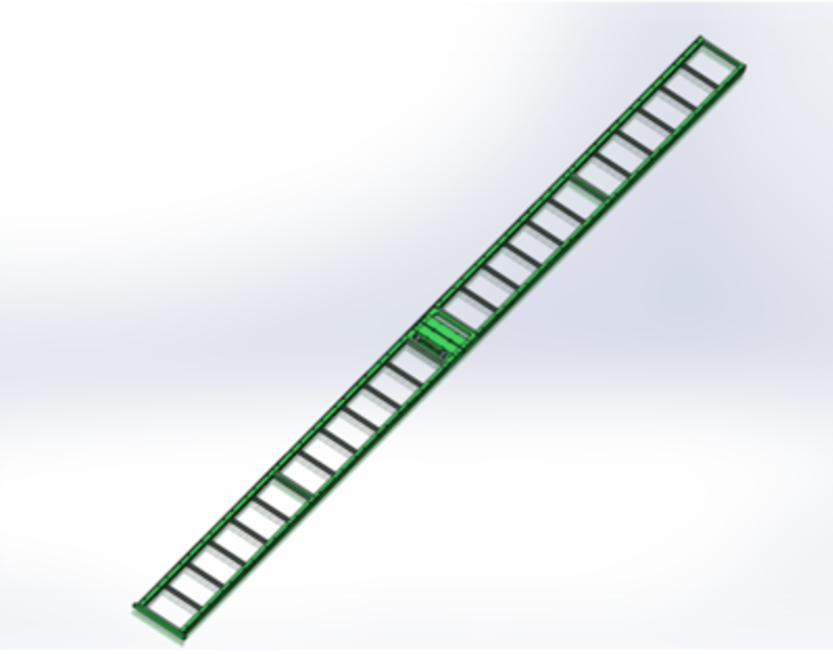
\includegraphics[width=0.49\textwidth]{PDBar.pdf}
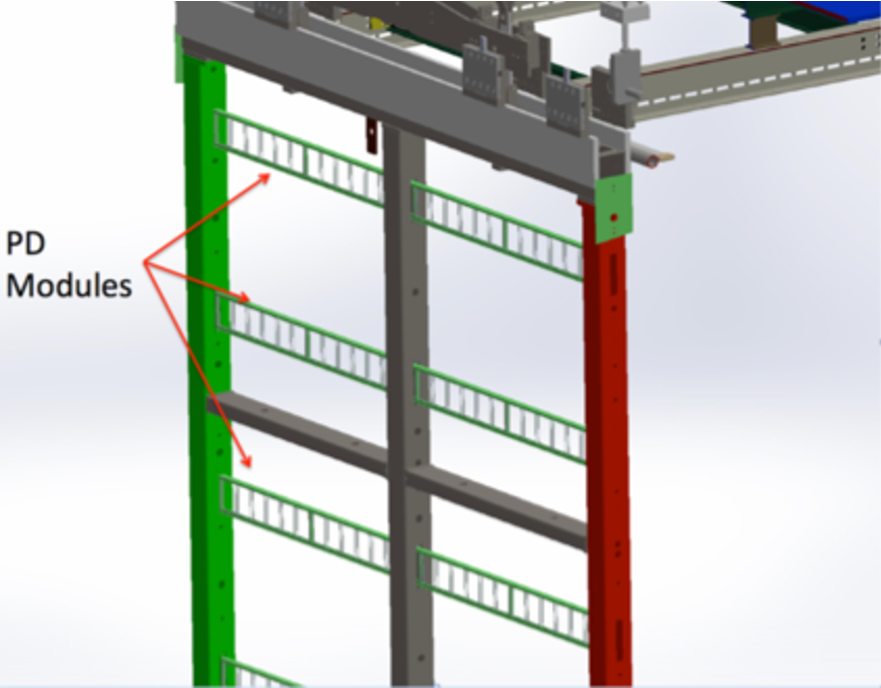
\includegraphics[width=0.49\textwidth]{PDsInAPA.pdf}
\end{dunefigure}

\begin{dunefigure}[An X-Arapuca photon-detector cell.]{fig:ArapucaCell}
{Left: an X-Arapuca cell. Right: an exploded view of the X-Arapuca cell, where the blue sheet is the wavelength-shifting plate and the yellow sheets the dichroic filters.}
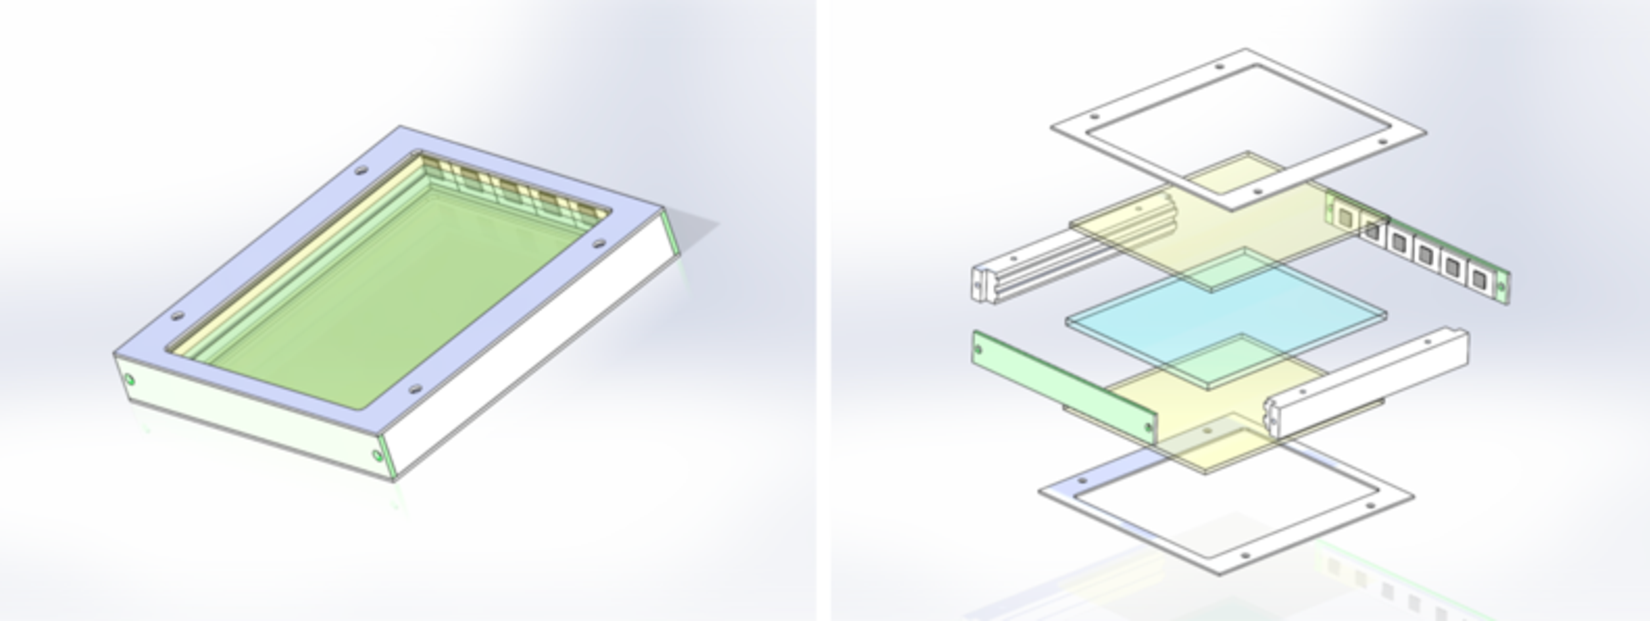
\includegraphics[width=\textwidth]{XArapuca.pdf}
\end{dunefigure}

The 48 \dword{sipm}s on each X-Arapuca supercell are ganged together and the signals are collected by front-end electronics, mounted on the supercell. The design of the front-end electronics is inspired by the system used for the Mu2e cosmic-ray tagger~\cite{bib:mu2e_tdr}, which uses commercial ultrasound \dword{asic}s. The front-end electronics define the \SI{1}{\micro\second} timing resolution of the \dword{pd} system.

\section{High Voltage, cathode planes and field cage}
\label{sec:fdsp-exec-hv}

The design voltage at which the \dword{dune} \dword{tpc} will operate is $-\SI{180}{\kilo\volt}$, corresponding to \SI{500}{\volt/\cm} across each drift volume. This voltage is a trade off. A higher voltage results in more charge collected, and hence better signal-to-noise ratio, better calorimetry, and lower detection thresholds, as well as less saturation of free charge at the point of ionization. A higher voltage, however, also reduces the amount of scintillation light produced and requires more space between the \dword{cpa}s and the cryostat walls to prevent discharges, reducing the fiducial volume. The \dword{protodune} experience shows that we can achieve this design voltage; nevertheless, from \dword{microboone}, we also know that a drift voltage of \SI{250}{\volt/\cm} achieves an adequate signal-to-noise ratio.

The \dword{hv} is supplied to the \dword{cpa} arrays. Each \dword{cpa} array (two per \SI{10}{\kilo\tonne} module) has its own independent high voltage supply. These commercial high voltage devices will supply a current of \SI{0.16}{\milli\ampere} at $-\SI{180}{\kilo\volt}$. The voltage is delivered, via $\sim\!\SI{30}{\meter}$ length commercial cables, through a series of few-\si{\mega\ohm} filtering resistors that act as low-pass filters to reduce noise and thereby satisfy the ripple-voltage requirement of $<\!\SI{0.9}{\milli\volt}$ on the \dword{cpa} array, which corresponds to a requirement of $<\!100\,e{-}$ of noise injected into the \dword{tpc} by the high-voltage system. The supply unit monitors the voltage and current every \SI{300}{\milli\second}; toroids mounted on the cables are sensitive to much faster changes in current and enable responses to current changes on a timescale of \SIrange{0.1}{10}{\micro\second}.

The high voltage passes into the cryostat through a feedthrough based on the ICARUS design~\cite{Icarus-T600}, the stainless steel conductor of which mates with the \dword{cpa} array via a spring-loaded feedthrough.
When at $-\SI{180}{\kilo\volt}$, each \dword{cpa} array stores \SI{400}{\joule} of energy, so the \dword{cpa}s must have at least $\SI{1}{\mega\ohm/\cm^{2}}$ resistance to prevent damage if the field is quenched. The \dword{cpa}, an example of which from \dword{protodune} is shown in Figure~\ref{fig:CPA}, is a $\SI{1.2}{\meter}\times\SI{4}{\meter}$ planar unit, each side of which is a \SI{3}{\mm} thick FR-4 sheet, onto which is laminated a thin layer of carbon-impregnated Kapton that forms the resistive cathode plane.

\begin{dunefigure}[A ProtoDUNE cathode plane assembly.]{fig:CPA}
{A ProtoDUNE cathode plane assembly. The black surface is the carbon-impregnated kapton resistive cathode plane.}
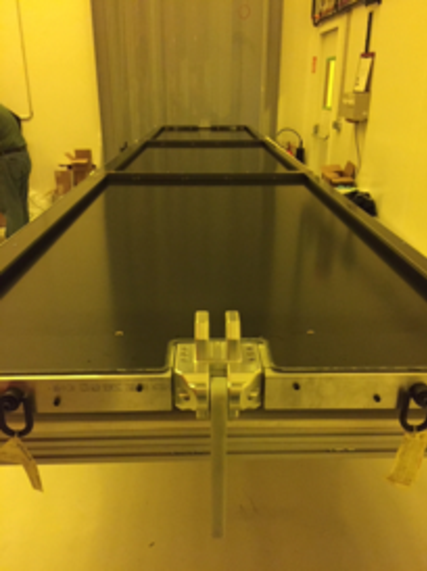
\includegraphics[width=0.35\textwidth]{CPA.pdf}
\end{dunefigure}

The field must be uniform throughout the active \dword{tpc} volume to within 1\%, and this is achieved by a \dword{fc} that surrounds the drift volumes. The \dword{fc} is built from field-shaping aluminum profiles, terminated with \SI{6}{\mm} thick ultra-high molecular-weight polyethylene caps (see Figure~\ref{fig:FieldCage}). All surfaces on these profiles must be smooth to keep local fields below \SI{30}{\kilo\volt/\cm}, a requirement that reduces the possibility of voltage breakdowns in the argon; the shape of the profiles leads to a maximum local field near the surface of the \dword{fc} of $\sim\!\SI{12}{\kilo\volt/\cm}$. The aluminum profiles are connected together via a resistive divider chain; between each profile, two \SI{5}{\giga\ohm} resistors, arranged in parallel, provide a \SI{2.5}{\giga\ohm} resistance to create a nominal \SI{3}{\kilo\volt} drop.

\begin{dunefigure}[A section of the field cage.]{fig:FieldCage}
{A section of the field cage, showing the extruded aluminium field-shaping profiles, with white polyethylene caps on the ends to prevent discharges.}
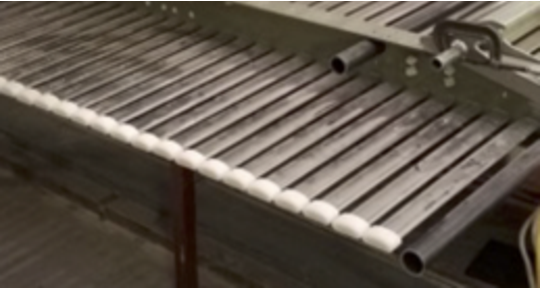
\includegraphics[width=0.5\textwidth]{FieldCage.pdf}
\end{dunefigure}

\section{Anode Planes}
\label{sec:fdsp-exec-apas}

The \dword{apa}s are $\SI{6}{\meter}\times\SI{2.3}{\meter}$ planes that form the three anode walls of the \dword{tpc}. An \dword{apa} is shown in Figure~\ref{fig:APA}. In the \dword{fd}, the \dword{apa}s are mounted in pairs, in portrait orientation, one above another, with the head end of the top \dword{apa} at the top of the detector and the head end of the bottom \dword{apa} at the bottom of the detector.

\begin{dunefigure}[An anode plane assembly.]{fig:APA}
{Top: a schematic of an anode plane assembly. In black is the steel \dword{apa} frame. The green and pink areas indicate the directions of the induction wire layers. The blue area indicates the directions of the induction and shielding (grid) wire layers. The blue boxes at the right-hand end  are the \dword{ce}. Bottom: a \dword{protodune} \dword{apa} in a wire-winding machine. The right-hand end of the \dword{apa} as shown in this picture is the head end, onto which the \dword{ce} are mounted.}
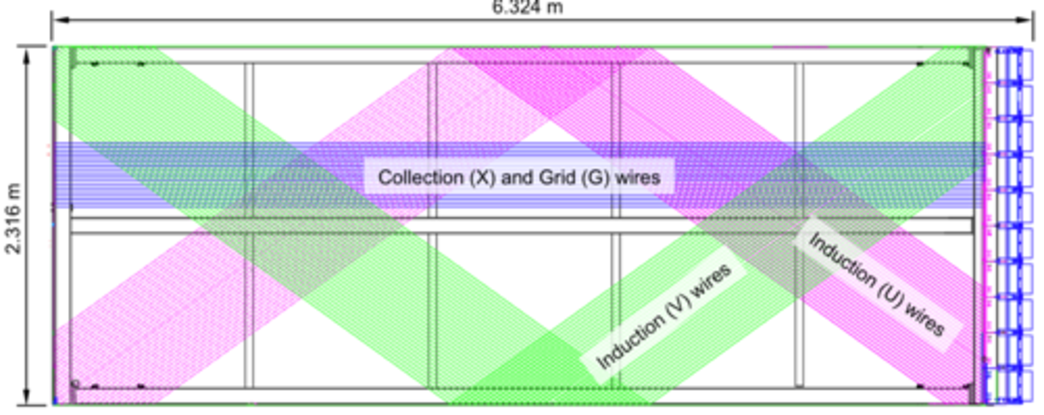
\includegraphics[width=0.7\textwidth]{APASchematic.pdf}
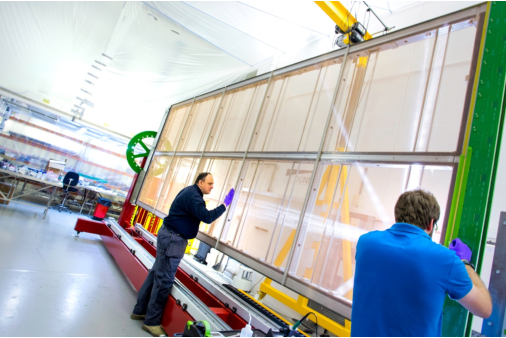
\includegraphics[width=0.6\textwidth]{RealAPA.pdf}
\end{dunefigure}

The basic building block of the \dword{apa} is the steel frame that can be seen outlined in Figure~\ref{fig:APA}, consisting of three long steel bars, a head shaft onto which the \dword{ce} are mounted, a foot shaft, and four thinner cross-braces. The two outer long sections are $4\,\mathrm{inch}\times 4\,\mathrm{inch}$ square-profile steel tubes through which run the \dword{pd} cables and the \dword{ce} cables from the bottom \dword{apa} of a pair. The \dword{pd}s are mounted into the \dword{apa}s, after production, through slots in these long sections.

Mounted directly onto both sides of the \dword{apa} frame is a grounding mesh, which ensures any ionization produced inside the \dword{apa} cannot cause signals on the active wire layers. The four wire layers, consisting of \SI{152}{\micro\meter} diameter copper-beryllium wire, are wound around the grounding mesh. The inside layer is the collection layer, called the $X$-layer, the 960 wires of which run parallel to the long axis of the \dword{apa}. Next are the two induction layers, the $U$- and $V$-layers, each with 800 wires at $\pm\SI{35.7}{\degree}$ to the long axis. Finally, the uninstrumented shielding layer, the $G$-layer, has 960 wires running parallel to the $X$-layer wires; this layer shields the three active layers from long-range induction effects. The wire spacing on each layer is \SI{4.79}{\mm} for the $X$ and $G$ layers and \SI{4.67}{\mm} for the $U$ and $V$ layers; the inter-plane spacing is \SI{4.75}{\mm}. The wire spacing on each plane defines the spatial resolution of the \dword{apa}; it is wide enough to keep readout costs low and signal-to-noise high, but small enough to enable reconstruction of short tracks such as few-\si{\cm} kaon tracks from proton-decay events. The tolerance both on the wire spacing in the plane and on the plane-to-plane spacing is \SI{0.5}{\mm}; this is most important in the plane-to-plane direction where the spacing ensures that the induction planes remain transparent to the drifting charge.

The wires are soldered to printed circuit boards located around the four sides of the \dword{apa}. These boards, shown in Figure~\ref{fig:GeometryBoardsAndCombs}, are called geometry boards since they define the wire spacing in all dimensions; they consist only of pads and traces: no active components. At the head end, these boards lie flat in the plane of the \dword{apa}, and the wires are terminated onto these boards for readout. On the remaining three sides, the boards sit on the sides of the \dword{apa}, perpendicular to the wire planes, and control the wrapping of the wires around the \dword{apa}. These wrap boards have insulating pins on their edges, around which the wires are wrapped, to set the wire spacing. At the head end, additional active boards are installed after all wires are wound: $G$-bias boards provide the necessary capacitance to the $G$-layer and a resistor to provide the bias voltage; $CR$-boards provide the interface between the $X$ and $U$ layers and the \dword{ce}, resistors providing the bias voltages and capacitors providing DC blocking. Relative to the ground, the four wire layers are biased to \SI{820}{\volt} ($X$-layer), \SI{0}{\volt} ($V$-layer), \SI{-370}{\volt} ($U$-layer), and \SI{-665}{\volt} ($G$-layer). To maintain the wire spacing across the \dword{apa}, wire-support combs, also shown in Figure~\ref{fig:GeometryBoardsAndCombs}, run along the four cross-braces across the short dimension of the \dword{apa}.

\begin{dunefigure}[Geometry boards and wire-support combs on an anode plane assembly.]{fig:GeometryBoardsAndCombs}
{Left: $V$-layer geometry boards, showing the head-end boards face-on and the wrap boards along the bottom. Back plastic insulating pins are visible on the edges of the wrap boards. The $V$-layer wires can be seen running diagonally, and the $X$-layer wires, horizontal in this picture, are visible behind those.  Right: wire-support combs, showing all four layers of wires.}
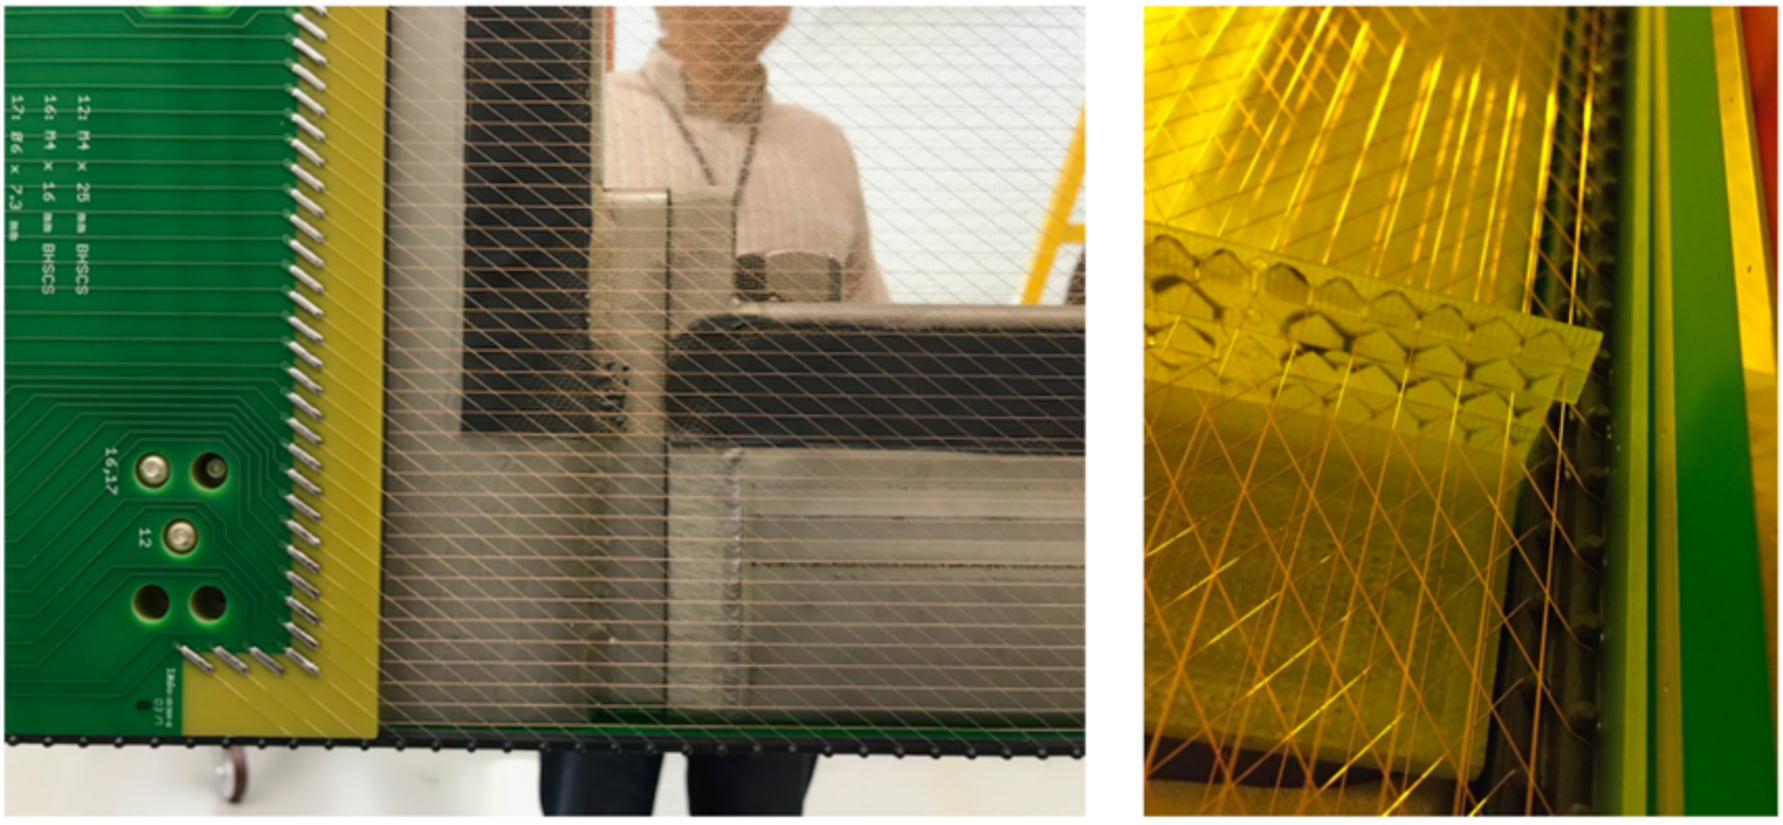
\includegraphics[width=\textwidth]{GeometryBoardsAndCombs.pdf}
\end{dunefigure}

%In the \dword{fd}, \dword{apa}s are hung in pairs, one above another, the bottom \dword{apa} hanging from the top \dword{apa}, as was shown in Figure~\ref{fig:APAStack}. Each \dword{apa} must be electrically isolated from all its neighbors, so the mechanical linkages use parts made from G10.

\section{Electronics}
\label{sec:fdsp-exec-electronics}

The job of the readout electronics is to send out of the cryostat digitized waveforms from the \dword{apa} wires. To enable us to look at low-energy particles, we aim to keep noise to below $1000\,e^{-}$ per channel, which should be compared to the $20k$--$30k\,e^{-}$ per channel collected from a minimum-ionizing particle traveling parallel to the wire plane and perpendicular to the wire orientation. For large signals, we require a linear response up to $500k\,e^{-}$, which ensures that fewer than 10\% of beam events experience saturation. This can be achieved using 12\, \dword{adc} bits. In addition, the electronics are designed with a front-end peaking time of \SI{1}{\micro\second}, which matches the time for the electrons to drift between wires planes on the \dword{apa}; this then leads to a design sampling frequency of \SI{2}{\mega\hertz} to satisfy the Nyquist criterion.

The digitization electronics are mounted on the head ends of the \dword{apa}s in the \dword{lar} and are therefore referred to as \dword{ce}. The low, \SI{87}{\kelvin} temperatures reduce thermal noise. Figure~\ref{fig:ElectronicsBlockDiagram} shows a block diagram of the \dword{femb}s mounted on the \dword{apa}s. Each \dword{apa} is instrumented with 20 \dword{femb}s, each of which takes the signals from 40 $U$-layer wires, 40 $V$-layer wires, and 48 $X$-layer wires. The signals pass through a series of three \dword{asic}s. The first \dword{asic}, the front-end \dword{asic}, shapes and amplifies the signals. The next \dword{asic}, the \dword{adc} \dword{asic}, performs the analogue-to-digital conversion. Finally, a \dword{coldata} \dword{asic} merges the datastreams from the preceding \dword{asic}s for transmission to the outside world; this \dword{coldata} \dword{asic} also controls the front-end motherboard and facilitates communications between the motherboard and the outside world.

\begin{dunefigure}[A block diagram of the anode-plane readout electronics.]{fig:ElectronicsBlockDiagram}
{Left: an \dword{apa} with 20 \dword{femb}s installed on the head end. Right: a block diagram of the readout electronics mounted on the APAs.}
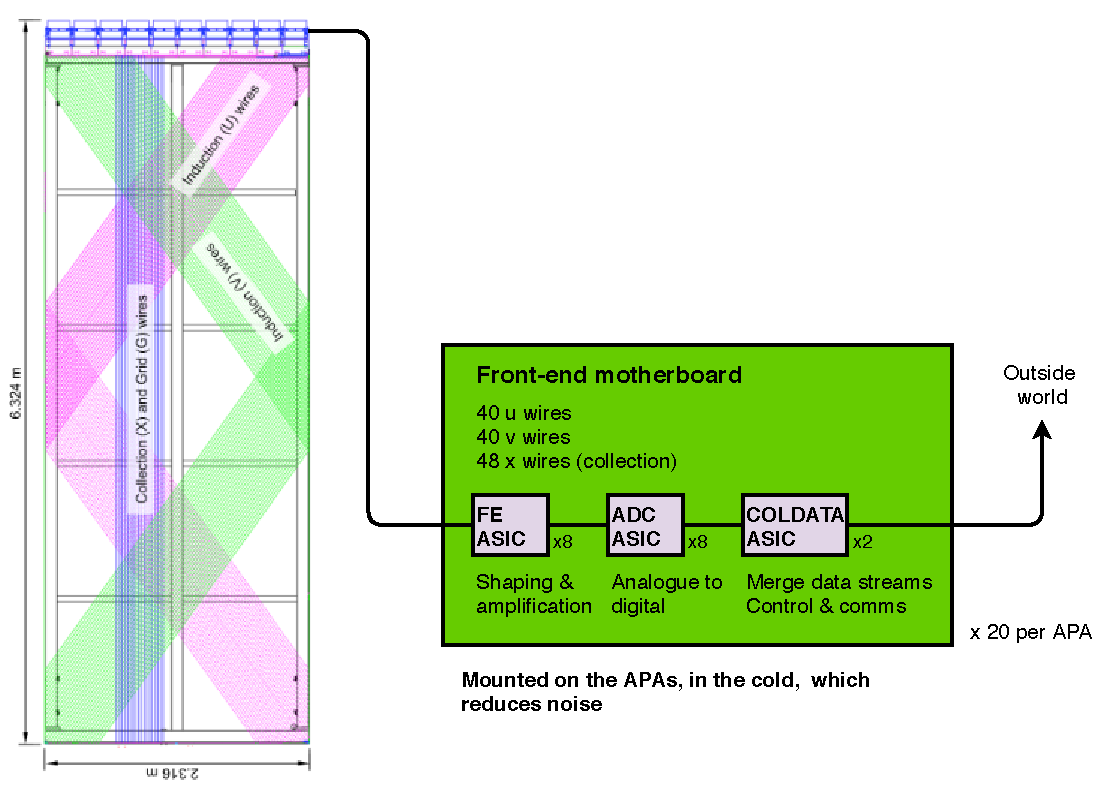
\includegraphics[width=0.8\textwidth]{ElectronicsBlockDiagram.pdf}
\end{dunefigure}

The data passes out of the cryostat through feedthroughs in the roof. Mounted directly to each feedthrough is a \dword{wiec}. Each \dword{wiec} contains five \dword{wib}s, each of which processes the signals from five \dword{femb}s. A \dword{wiec} also contains a \dword{ptc} that provides the fibre interface to the timing system, fanning out timing and control systems, as well as the low-voltage power, to the \dword{wib}s via a \dword{ptb}.

\section{Data Acquisition}
\label{sec:fdsp-exec-daq}


The \dword{daq} is divided between an upstream section, located underground in the \dword{cuc}, and a downstream \dword{daqbes} above ground at \dword{surf}. All trigger decisions are made underground, and the data buffered underground until the \dword{daqbes} indicates it is ready to receive data, in order to minimize the rate of data flowing to the surface. An end-goal of the \dword{daq} is to achieve a data-rate to tape of no more than \SI{30}{\peta\byte/\year}.

The \dword{daq} architechture is based on the \dword{felix} system designed at \dword{cern} and used for the LHC
%\fixme{This abbreviation (LHC) is not in the common glossary.} 
experiments. The 150 \dword{apa}s from each \SI{10}{\kilo\tonne} module are processed by 75 \dword{daqrou}; each \dword{daqrou} contains one \dword{felix} board. The \dword{pd}s from the module will have a lower data-rate since the \dword{pd} electronics, unlike that of the \dword{tpc}, perform zero-suppression; therefore the \dword{pd}s of a module will be processed by six to eight additional \dword{daqrou}s. The \dword{daq} will be partitionable: it will be possible to run multiple instances of the \dword{daq} simultaneously so that the majority of the detector can be taking physics data whilst other \dword{daq} instances are running test runs for development or special runs such as calibration runs. A key philosophy is that all the primary \dword{dune} physics goals can be achieved using only the \dword{tpc} as the trigger; information from the \dword{pd}s can then further enhance the trigger.

There will be two basic triggers operating. Beam, cosmic and nucleon decay events will be triggered using the localized high-energy trigger. This will trigger on localized regions of visible activity, for example in a single \dword{apa}, with a $>99\%$ trigger efficiency at \SI{100}{\mega\electronvolt} and a trigger threshold as low as \SI{10}{\mega\electronvolt}. A localized high-energy trigger will open a readout window of \SI{5.4}{\ms}, enough to readout the full TPC drift around an event. For \dword{snb}s, we will use an extended low-energy trigger. This will look for coincident regions of low-energy deposits, below \SI{10}{\mega\electronvolt}, across an entire module and in a \SI{10}{\second} period. An extended high-energy trigger will open a readout window of \SI{100}{\second} to capture a full \dword{snb}. The upstream \dword{daq} identifies per-channel regions of interest and forms them into trigger primitives. These are then formed into trigger candidates that contain information from an entire module; on these trigger candidates, trigger decisions are made. Once a trigger decision has been made, this will be communicated to the surface, and the data buffered underground until the \dword{daqbes} indicates it is ready to receive data.

The \dword{daq} must also provide the system clock that keeps the detector components synchronized and provides the timestamp for all data. The timestamp derives from a \dword{gps} \dword{pps} that is fed into the \dword{daq} with \SI{1}{\micro\second} precision, adequate to timestamp beam and supernova events. To provide the finer synchronization between detector components, a \SI{10}{\mega\hertz} reference clock drives the module's \SI{62.5}{\mega\hertz} masterclock, which is fanned out to all detector components, providing an overall synchronization to a precision of \SI{1}{\nano\second}.

\section{Calibration}
\label{sec:fdsp-exec-calibration}

The challenge of calibrating the \dword{dune} \dword{fd} is to control the response of a huge cryogenic detector over a period of decades, a challenge amplified by the detector's location deep underground and therefore shielded from the cosmic muons that were typically used as standard candles by previous \dword{lartpc}s.

To achieve our $\mathcal{O}(\si{\giga\electronvolt})$ oscillation and nucleon decay physics goals, we must know our fiducial volume to 1--2\% and have a similar understanding of the vertex position resolution; understand the \nue event rate to 2\%; and control our lepton and hadron energy scales to 1\% and 3\%, respectively. At the $\mathcal{O}(\si{\mega\electronvolt})$ scale our physics requirements are driven by our goal of identifying, and measuring the spectral structure of, a \dword{snb}; here, we must achieve a 20--30\% energy resolution, understand our event timing to the \SI{1}{\micro\second} level, and measure our trigger efficiency and levels of radiological background. These are all high-level calibration requirements, but the underlying detector parameters that we are characterising are parameters such as the energy deposted per unit length ($\mathrm{d}E/\mathrm{d}x$), ionisation electron drift-lifetimes, scintillation light yield and detection efficiency, electric field maps, timing precision, \dword{tpc} alignment, and the behaviour (noise, gain, cross-talk, linearity, etc.) of electronics channels.

The tools available to us for calibration include the \dword{lbnf} beam, atmospheric neutrinos, atmospheric muons, radiological backgrounds, and dedicated calibration devices that will be installed in the detector. At the lowest energies, we have deployable neutron sources and intrinsic radioactive sources; in particular the natural $^{39}$Ar component of the \dword{lar} with its \SI{565}{\kilo\electronvolt} end-point can, given its pervasive nature across the detector, be used to measure the spatial and temporal variations in electron lifetime. The possibility of deploying radioactive sources is also being explored. In the \SIrange{10}{100}{\mega\electronvolt} energy range we will use Michel electrons, photons from $\pi^{0}$ decay, stopping protons and both stopping and through-going muons. We will also have built-in lasers, purity monitors and thermometers, and the ability to inject charge into the readout electronics. Finally, data from the \dword{protodune} detectors will be invaluable in understanding the response and particle-identification capabilities of the \dword{fd}.

Once the first \SI{10}{\kilo\tonne} module is switched on, there will be a period of years before \dword{lbnf} beam sources are available for calibration --- and even then the statistics will be limited. In this time, cosmic muons will be available, but the low rate of these means that it will take months to years to build up the necessary statistics for calibration. The inclusive cosmic muon rate for each \SI{10}{\kilo\tonne} module is $1.3\times 10^{6}$ per year. However, for calibrations such as \dword{apa} alignment, the typical rate of useful muons is 3000--4000 per APA per year. For energy-scale calibrations, stopping cosmic muons are the most relevant and here the rate is 11000 per \SI{10}{\kilo\tonne} module per year. Therefore the earliest calibrations will come from dedicated calibration hardware systems and intrinsic radiological sources.

A \SI{266}{\nano\meter} laser will be used to ionise the argon, and this can be used to map the electric field and to make early measurements of \dword{apa} alignment. The laser system will be used throughout the lifetime of the detector to measure the gradual changes in the electric field map as positive ions accumulate and flow around the detector.
%The natural $^{39}$Ar $\beta$-decay rate in commercial argon is $\sim\!\SI{1}{\becquerel\,\kilo\gram^{-1}}$. With an end-point energy of \SI{565}{\kilo\electronvolt}, close to the energy deposited on a single wire by a \dword{mip}, the reconstructed energy spectrum and observed signal shapes can be used to measure the spatial and temporal variation of electron lifetime, the wire-to-wire response variations and the diffusion of ionisation.
An externally deployed pulsed neutron source provides a triggered, well-defined energy deposition from neutron capture in Ar which is an important component of signal processes for \dword{snb} and \dword{lbl} physics. A radioactive source deployment system, which is complementary to the pulsed neutron system, can provide at known locations inside the detector a source of gamma rays in the same energy range as \dword{snb} and solar neutrino physics

Over time, the \dword{fd} calibration programme will evolve as statistics from the cosmic rays and the \dword{lbnf} beam amass and add to the information gained from the calibration hardware systems. These numerous calibration tools will work alongside the detector monitoring system, the computational fluid dynamics models of the argon flow, and \dword{protodune} data to give us a detailed understanding of the \dword{fd} response across the \dword{dune} physics programme.


\section{Installation}

A major challenge in building the \dword{dune} \dword{sp} modules is transporting all the detector and infrastructure components down the \SI{1500}{\meter} Ross shaft, to the detector caverns. To aid the planning of the installation phase, installation tests will be performed at Ash River. These tests will allow us to develop our procedures, train the installation workers, and develop our labour planning through time and motion studies.

Once the module's cryostat has been installed, a \dword{tco} is left open at one end through which the detector components are installed. A cleanroom is built around the \dword{tco} to prevent any contamination entering the cryostat during installation. The \dword{dss} is then installed into the cryostat, ready to receive the \dword{tpc} components. 

Inside the cryostat, the various monitor devices (temperature, purity, argon level) are installed at the end furthest from the \dword{tco}. The far end of the \dword{fc} is then installed. Rows of \dword{apa}s and \dword{cpa}s, along with the top and bottom \dword{fc} sections, are then installed and cabled, working from the far end of the detector towards the \dword{tco}. The integration of the \dword{pd}s and \dword{ce} with the \dword{apa} happens in the cleanroom immediately outside the \dword{tco}. Finally, the second \dword{fc} end-wall is installed across the \dword{tco}, along with the monitoring devices at the \dword{tco} end. The \dword{tco} can then be closed up and the cryostat is ready to purge and fill with \dword{lar}. The warm electronics and \dword{daq} are installed in parallel with the \dword{tpc} installation.

Throughout the installation process, safety is the paramount consideration: safety both of personnel and of the detector components. Once the detectors are taking data, safety is still the priority with the \dword{ddss} monitoring for argon level drops, water leaks and smoke. A detailed detector and cavern grounding scheme has been developed that not only guards against ground loops, but also ensures that any power faults are safely shunted to the facility ground.

Throughout the project, \dword{qa} and \dword{qc} are written into all processes. Most detector components are constructed off-site at collaborating institutions; strict \dword{qc} procedures will be followed at all production sites to ensure that components are working within specifications before delivery to \dword{surf}. Underground at \dword{surf} integrated detector components are tested in the cleanroom to ensure functionality, before passing them through the \dword{tco} for installation. Finally, \dword{qc} is performed on all integrated components inside the cryostat, in particular to ensure that all connections have been made through to the \dword{cuc}.

\section{Conclusion}
\label{sec:fdsp-exec-conclusion}

This executive summary has provided an overview of the design of the \SI{10}{\kilo\tonne} \dword{sp} \dword{lartpc} modules of the \dword{dune} \dword{fd}, explaining how key design choices have been made to ensure we can achieve our primary physics goals of searching for leptonic $CP$ violation, nucleon decay and neutrinos from supernova bursts. The chapters that follow go into significantly more detail about the design of the \dword{sp} \dword{fd} modules. In addition to describing the design and requirements, these chapters include details on the construction, integration and installation procedures, the \dword{qa} and \dword{qc} processes that have been developed to ensure that the detector will function for a period of decades, and the overall project management structure. The chapters also describe how the design has been validated and informed by \dword{protodune}.

